\documentclass{beamer}

\usepackage[utf8]{inputenc}
\defbeamertemplate{description item}{align left}{\insertdescriptionitem\hfill}

\usepackage{hyperref}
\hypersetup{
    colorlinks=true,
    linkcolor=blue,
    filecolor=magenta,      
    urlcolor=cyan,
}



%Information to be included in the title page:
\title{311 Social Distancing NYC}
\subtitle{Exam project for Management of Scientific Data}
\author{Anna Sterzik}
\institute{Friedrich Schiller Universität Jena}
\date{\today}



\begin{document}

\frame{\titlepage}
\begin{frame}
\frametitle{Table of Contents}
\tableofcontents
\end{frame}

\section{Data Management Plan}
\begin{frame}
\frametitle{Project Information}
\setbeamertemplate{description item}[default]
\begin{description}[style=multiline]
\item[Project name:] 311 Social Distancing NYC
\vfill
\item[Creator:] Anna Sterzik
\vfill
\item[Affiliation:] Friedrich Schiller University Jena
\vfill
\item[Template:] DCC Template
%Project abstract:
%The 311 Service Requests in New York City will be used to investigate how the acceptance of Social Distancing
%measures evolved during the Covid-19 pandemic in New York City. Therefore violations of Social Distancing rules
%will be analysed over time.
Last modified: 10-08-2020
\item The tool \href{https://dmponline.dcc.ac.uk/}{DMPonline} was used
\end{description}

\end{frame}
\begin{frame}
\frametitle{Preexisting Data}
\begin{itemize}
\item Pre-existing data from \href{https://data.cityofnewyork.us/Social-Services/311-Service-Requests-from-2010-to-Present/erm2-nwe9}{311 Service Requests from 2010 to Present}.
\vfill
\item Initial Data Filtering:
\setbeamertemplate{description item}[align left]
\begin{description}[style = multiline]
\item [Description:] Including "Social Distancing"
\end{description}
\vfill
\item raw data volume: 32.8 MB
\vfill
\item Data Format: CSV
\vfill
\item Open Data \url{https://opendata.cityofnewyork.us/faq/}
\vfill
\item Accessed/Downloaded 2020-08-11
\end{itemize}
\end{frame}
\begin{frame}
\frametitle{Generated Data}
\begin{itemize}

\item Data Quality will be monitored using \href{https://openrefine.org/}{OpenRefine}. For every version of refined data the OpenRefine project will be saved together with a version number.
\vfill
\item Data will be analyzed and visualized using jupyter notebooks. 
\vfill
\item Formats: TXT, JSON, PDF, PNG, TEX, IPYNB
\vfill
\item Everything apart from raw data will be put under version control by using git.
\end{itemize}
\end{frame}

\begin{frame}
\frametitle{Documentation and Metadata}
\begin{itemize}
\item Software versions used for this project:
\setbeamertemplate{description item}[align left]
\begin{description}
\item[OpenRefine:] 3.3
\item[Python: ] 3.7.4
\item[Pandas: ] 0.25.1
\item[Jupyter: ] 1.0.0
\item[Matplotlib: ] 3.1.1
\item[Numpy: ] 1.17.4 
\end{description}
\vfill
\item Documentation will be provided as a README
\vfill
\item Provenance for Data Cleansing by usage of OpenRefine
\vfill
\item Provenance for Jupyter Notebooks will be handled by \href{https://github.com/Sheeba-Samuel/ProvBook}{ProvBook}
\end{itemize}
\end{frame}

\begin{frame}
\frametitle{Storage and Backup}
\begin{itemize}
\item Project will be hosted on github and additional backup will be with URZ and on a USB stick
\vfill
\item Data will be available for everyone at all times via github.
\end{itemize}
\end{frame}
\begin{frame}
\frametitle{Selection, Preservation and Sharing}
\begin{itemize}
\item The created software for analysis as well as the steps during data cleaning are essential part. The third party data is already preserved.
\vfill
\item The project will be hosted on github and will be available under a MIT licence.
\end{itemize}
\end{frame}
\begin{frame}
\frametitle{Resources}
\begin{itemize}
\item The only ressources required are storage capacity from URZ.
\end{itemize}
\end{frame}
\section{Description of the Dataset}
\begin{frame}
\frametitle{Description of the Dataset}
311 Service Requests in New York City from 2010 to present
\vfill
\begin{itemize}
\item Non-emergency social service requests
\vfill
\item Provider: DoITT Department of Information Technology \& Telecommunications
\vfill
\item Owner: NYC OpenData
\vfill
\item There are 41 columns in the dataset, they include but are not limited to unique key, information about time, agency, complaint type, location information
\item Each row is a service request
\end{itemize}
\end{frame}
\section{Quality Control}
\begin{frame}
\frametitle{Quality Control}

\begin{itemize}
\item Quality control will be done using \href{https://openrefine.org/}{OpenRefine}
\vfill
\item The database states:\\
``NOTE: This data does not present a full picture of 311 calls or service requests, in part because of operational and system complexities associated with remote call taking necessitated by the unprecedented volume 311 is handling during the Covid-19 crisis. The City is working to address this issue.''
\vfill
\item One can also see at first glance that there are several missing values
\end{itemize}
\end{frame}
\begin{frame}

\frametitle{Facets}
\begin{columns}
\column{0.5\textwidth}
Facets can be used to get a better overview over the data in specific columns.
The Complaint Types and Agency Names seem to be reasonible.
\column{0.5\textwidth}
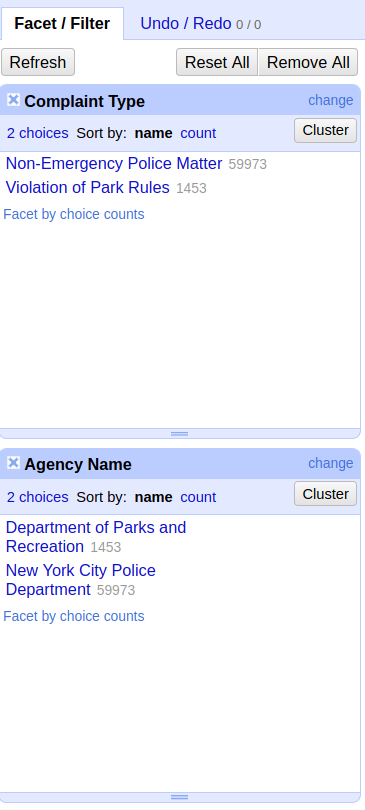
\includegraphics[width = 0.8\textwidth]{pictures/facets.png}
\end{columns}
\end{frame}
\begin{frame}
\frametitle{Clustering}
Clustering is another option to identify erronous data, especially spelling mistakes.
\vfill
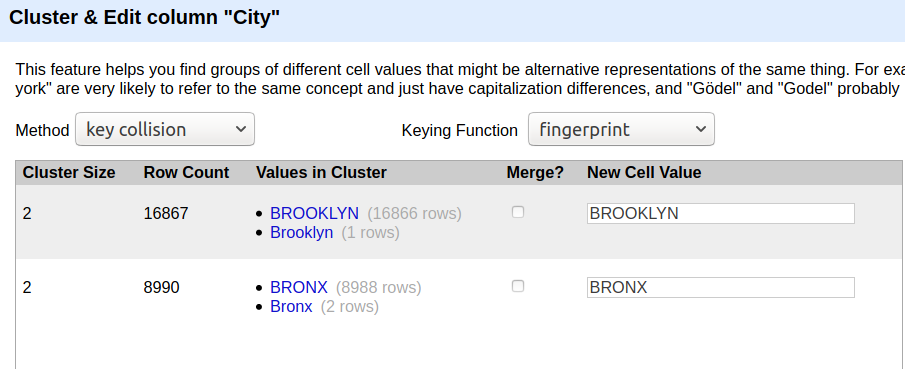
\includegraphics[width = \textwidth]{pictures/clustering.png}
\end{frame}
\begin{frame}
\frametitle{Sorting}
Using OpenRefine one can also sort the values by certain columns. That way one can e.g. determine if the given longitudes and latitudes are reasonable.
Here the latitudes and longitudes seem to be valid for NYC.
\vfill
The same can be done for the dates. The creating dates for example start with 2020-03-28 and end with 2020-08-10. This seems to be right as well, because PAUSE started at 2020-03-22.
\vfill
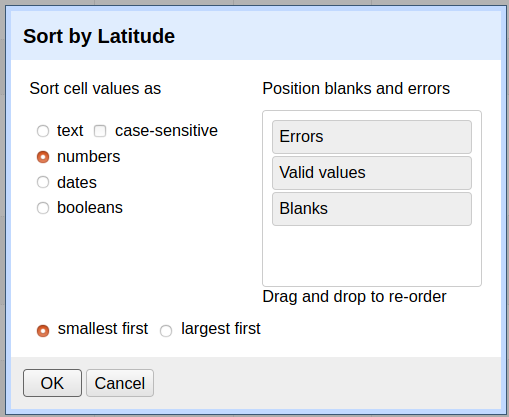
\includegraphics[width=0.5\textwidth]{pictures/sorting.png}
\end{frame}
\begin{frame}
\frametitle{Saving}
OpenRefine projects can be exported. The resulting files do only contain TXT files and JSON files. These files describe all changes made with the data.
\end{frame}
\section{Data analysis}
\begin{frame}
\frametitle{Data Analysis}
Data analysis will be done using pandas library in a jupyter notebook environment.
\end{frame}
\begin{frame}
\frametitle{Number of Service Calls about 'Social Distancing' in calendar weeks}

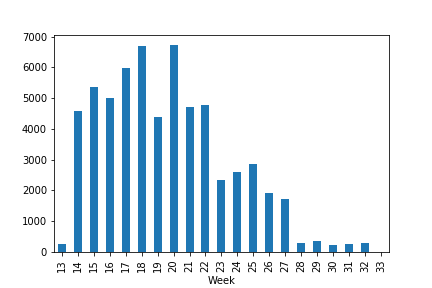
\includegraphics[width=\textwidth]{pictures/bar.png}

\end{frame}
\begin{frame}
\frametitle{Comparison of 'Social Distancing' Service Calls in Bronx and Manhattans}

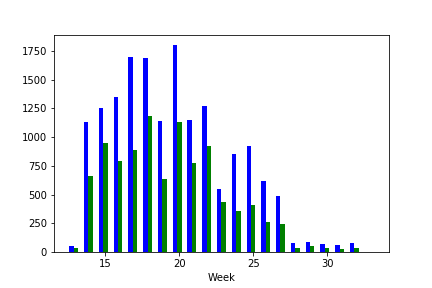
\includegraphics[width=\textwidth]{pictures/comp_bronx_manhattan.png}

\end{frame}
\section{Preservation and Publishing}
\begin{frame}
\begin{itemize}
\frametitle{Preservation and Publishing}
\item Publishing on Github: \url{github.com/azuki-monster/311-Service-Calls-NYC}
\vfill
\item Backup copies with the URZ and a USB drive as well
\vfill
\item Material available on Github under a MIT Licence
\end{itemize}
\end{frame}

\end{document}